Because our study includes individuals who experienced the Reggio Approach as well as others who experienced alternative early childhood programs, it is important to examine the similarities and differences between the available programs. This section documents the Reggio Approach in addition to exploring the extent to which other programs adopted innovative features of the Reggio Approach at different points of time.

To increase our understanding of the evolution of the programs listed in Table~\ref{tab:itc-pre}, we collected historical records from Reggio Emilia, Reggio Children, and Padova\footnote{We were unsuccessful in sourcing historical records from Parma.} \citep{Padova-Admin-Data_1964-2011,Reggio-Admin-data_1966-2006,Reggio-Annual-Journals_1994-2011} and administered a historical survey to current and former school administrators and educative coordinators in order to quantify pedagogical and administrative features of early childhood programs available during 1950-2010 \citep{CEHD_2016_Historical-Analysis}.\footnote{See Appendix~\ref{sec:survey} for the full survey.} 
~\\
\begin{table}[H]
\centering
\caption{Availability of Preschool Programs by City and School Type}\label{tab:itc-pre}
\begin{adjustbox}{width=\textwidth}
\begin{threeparttable}
	\begin{tabular}{l l c c c c c c c c c}
\toprule
\mc{1}{c}{Cohort} & \mc{3}{c}{Years} & \mc{3}{c}{Reggio Emilia} & \mc{3}{c}{Parma} & \mc{3}{c}{Padova} \\
& Municipal & Catholic & State & Municipal & Catholic-private & State & Municipal & Catholic-private & State \\
\midrule
Adults 50s & 1957-1965 & & \checkmark & & & \checkmark & & & \checkmark & \\
Adults 40s & 1972-1976 & \checkmark & \checkmark & & & \checkmark & & & \checkmark & \\
Adults 30s & 1983-1987 & \checkmark & \checkmark & \checkmark & \checkmark & \checkmark & \checkmark & \checkmark & \checkmark & \checkmark \\
Adolescents & 1994-2000 & \checkmark & \checkmark & \checkmark & \checkmark & \checkmark & \checkmark & \checkmark & \checkmark & \checkmark \\
Children & 2009-2014 & \checkmark & \checkmark & \checkmark & \checkmark & \checkmark & \checkmark & \checkmark & \checkmark & \checkmark \\
\bottomrule
\end{tabular}
\begin{tablenotes}
Note: This table indicates the majority of educational preschool systems available to parents in each city during the years each cohort was between 3 and 6 years old. 
\end{tablenotes}
\end{threeparttable}
\end{adjustbox}
\end{table}

The survey was designed to explore the extent to which notable administrative and pedagogical components of the Reggio Approach were present in state and religious systems at different points of time. The components included in the survey were identified by published program descriptions and confirmed by scholars with expertise in  the Reggio Approach and early childhood programs in Northern Italy.\footnote{See \citet{Edwards-etal-eds_1998_Hundred-Languages} and \citet{Corsaro_2008_Policy-Practice}.} The list of components include various aspects of administrative program operations such as staffing, supervision, enrollment, and funding. It also considers pedagogy and educational practices for children's learning and parental engagement. Respondents were asked to indicate whether the components of the survey were present in their systems during different decades. Additional questions were included to understand sources of funding and services for immigrant families.\footnote{For a more detailed summary of the items and the responses, see Appendix \ref{sec:survey}.} Table~\ref{tab:respondents} identifies the school systems in each city that completed our survey.

\begin{table}[H]
\centering
\caption{Survey Respondents by City and School Type}\label{tab:respondents}
\begin{threeparttable}
	\begin{tabular}{lccc}
\toprule
City & Municipal & State & Religious \\
\midrule
Reggio Emilia & \checkmark & \checkmark & \\
Parma		& \checkmark & & \\
Padova & \checkmark & \checkmark & \checkmark \\
\bottomrule
\end{tabular}
\begin{tablenotes}
Note: This table indicates the systems represented by survey respondents. These individuals included current and former administrators and educative coordinators. One survey was provided by each system noted, but answers reflected the input of multiple people employed by the system. Responses were provided by religious systems in Reggio Emilia and Parma, however, they did not include historical data prior to 2000. 
\end{tablenotes}
\end{threeparttable}
\end{table}

Results from the historical survey indicate that early childhood education systems within Reggio Emilia, as well as in Parma and Padova, share a number of similar characteristics. These include features of program administration, various pedagogical methods, and practices for at-risk children and families. The general trend shows that programming and practices endorsed by the municipality of Reggio Emilia is increasingly present in other early childhood systems, albeit to different degrees and at different times. We interpret these results as potential evidence for spillovers into alternative treatments. We further interpret the outcomes as evidence of unique investment by the municipality of Reggio Emilia into innovative educational programs and services for early childhood in support of working families. Overall, we acknowledge the small sample of survey respondents is too limited to ensure reliability or validity of outcomes. We further acknowledge the design of our historical survey limits our ability to capture strengths of alternative systems. Finally, we caution that the historical survey should not be interpreted as a quality measure of early childhood systems.

To summarize our findings, we compare the different programs in Figures~\ref{fig:agg-admin} and~\ref{fig:agg-ped}. A more detailed description is provided in the section that follows. Using survey results, we calculate the number of administrative and pedagogical components that each program shared with the Reggio Approach by school type, city, and year. We examine 14 administrative components and 16 pedagogical components (not all of the pedagogical components were present in the Reggio Approach). Over time, many of the programs increasingly adopted pedagogical and administrative practices endorsed by the Reggio Approach. This is especially true for Parma's municipal program, and somewhat true for Padova's municipal program. The other systems did not adopt as many pedagogical components as they did administrative ones. Even though the Reggio Approach remains distinctive when considering the sum of its elements, many of the alternative schools evolved to include a substantial portion of the elements.

\begin{figure}[H]
\begin{center}
\begin{subfigure}[b]{0.49\textwidth}
	\caption{Number of Administrative Characteristics in Common with the Reggio Approach}\label{fig:agg-admin}
	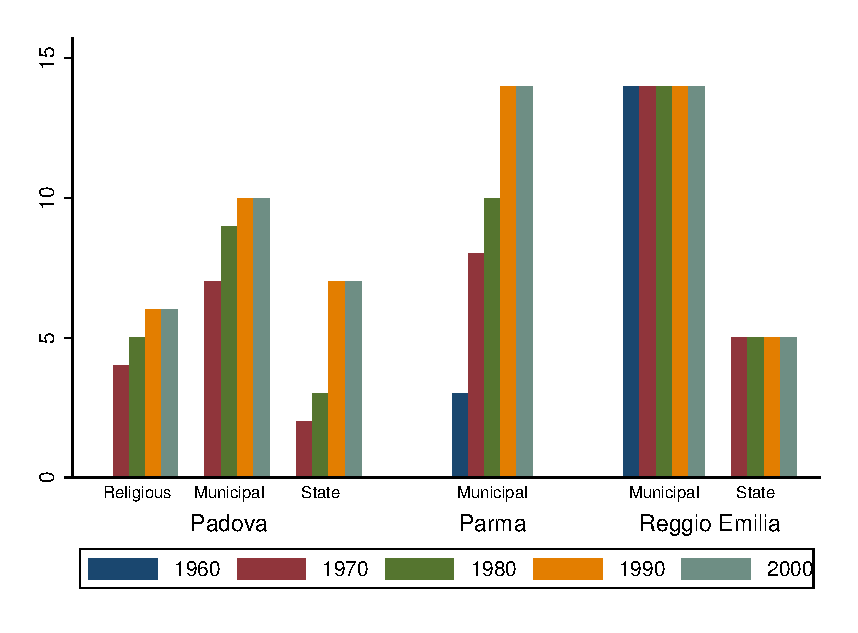
\includegraphics[width=\textwidth]{../../output/aggregateAdministrative.eps}
\end{subfigure}%
~
\begin{subfigure}[b]{0.49\textwidth}
	\caption{Number of Pedagogical Characteristics in Common with the Reggio Approach}\label{fig:agg-ped}
	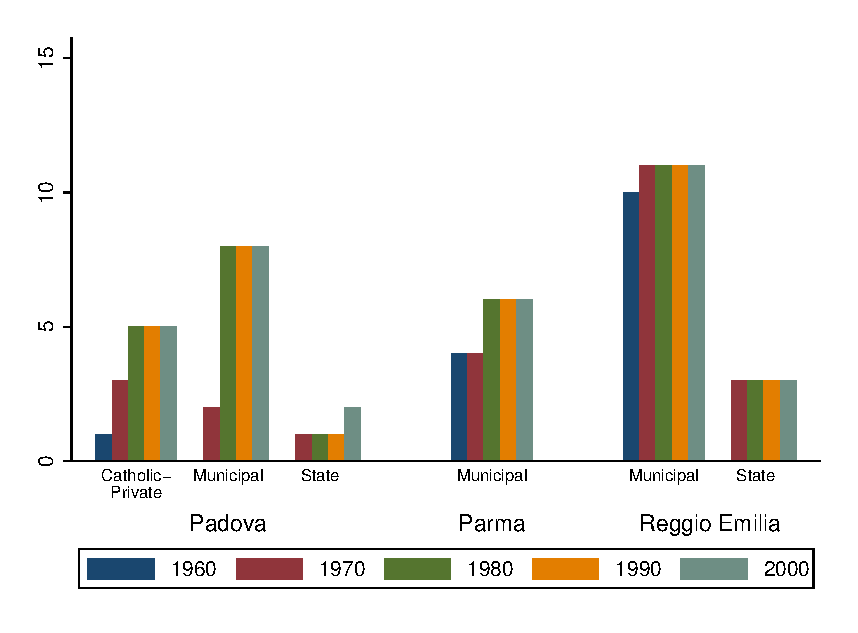
\includegraphics[width=\textwidth]{../../output/aggregatePedagogical.eps}
\end{subfigure}%
\end{center}
\raggedright \footnotesize Note: These graphs show the number of administrative and pedagogical components that each program has in common with the Reggio Approach. We consider 14 administrative components and 16 pedagogical components. Some of the pedagogical components were not present in the Reggio Approach. 
\end{figure}

%\footnote{See Appendix~\ref{} for more extensive discussion of the survey results.}

\subsection{Municipal Schools in Reggio Emilia - The Reggio Approach}

Of the municipal systems in Reggio Emilia, Parma, and Padova, the Reggio Approach is notable for its significant investment in innovative municipal programs and services. Of the three, it was the earliest municipal system to evolve and historically offers the largest number of municipal infant-toddler and preschool sites.\footnote{Similar to Parma and Padova, Reggio Emilia contracts with local private providers and cooperatives to offer infant-toddler and preschool slots according to municipal regulations. These ``affiliated'' programs may not follow the Reggio Approach nor the municipal approaches in Parma and Padova. Accordingly, we consider this a separate category during analysis.} While eligible, Reggio Emilia did not receive state funding for its municipal early childhood system until the 1990s and 2000s. Ironically, the municipality contributed funds to its local state schools each decade from the 1970s. In 1994, Reggio Approach staff provided training for religious preschool teachers in Reggio Emilia. 
% Maybe for the discussion? Last two sentences above

The Reggio Approach is a form of progressive early childhood education influenced by Loris Malaguzzi, an educator promoting the educational practices and psychological theories of Dewey, Piaget, Erikson, Vygotsky, Bronfenbrenner, Kagan, and Gardner. In 1963, Reggio Emilia opened its first preschool for children aged 3-6 years. In 1965, municipal policies were enacted to provide funding for infant-toddler centers for children aged 3 months to 3 years. The first of these infant-toddler centers was opened in 1971. Reggio Emilia's municipal early childhood system preceded Italy's key legislative reforms that established state-run preschools and mandated the local provision of infant-toddler centers \citep{Cagliari-etal-eds_2016_BOOK_Loris-Malaguzzi}. The Reggio Approach views curriculum as an ongoing, collaborative project without pre-determined learning goals or timelines. There is no institutionally-prescribed content knowledge that educators convey to children for ``school readiness.'' In contrast, teachers and children are viewed as researchers and co-creators of knowledge. For example, educators, children and families collaborate to define a question or topic. Learning is then pursued following a scientific process: theories are shared, tested, and revised through dialogue. 

In Reggio Approach preschools, the educative team is assigned specialized roles. Each incoming class of approximately 25 3-year-olds is assigned two full-time co-teachers. At least 1 of the 2 teachers remains with this cohort of homogeneous-aged children for three consecutive years. This extended time provides continuity of care for children and enables strong teacher-family engagement. Each preschool site is further staffed by a full-time atelierista, an instructor with a background in visual arts. Teachers observe children's development, interact with children through questions and dialogue, and provide scaffolding to support learning. Children demonstrate their emerging knowledge through creative learning activities and art, with aid from the atelierista. Teachers document each child's development in a portfolio that is shared and discussed with children and parents over the year \citep{Rinaldi_2006_ReggioEmilia_BOOK,Giudici-Nicolosi_2014_Reggio-Approach}. Auxiliary site staff, such as cooks and janitors, are considered members of the educative team and participate in trainings and professional development. A pedagogista, or educative coordinator, with a higher degree in psychology or education is assigned to support professional development on a biweekly basis for the educative staff of approximately 4-5 municipal preschools. 

The Reggio Approach school environment reflects a light-filled, open interior design, furnished with natural materials and a garden. Each site is equipped with an atelier, or dedicated studio laboratory used for creative instructional activities. In-house kitchens are surrounded by glass walls, to include children in the meal process, and is used daily for preparing meals. Reggio Approach preschools and infant-toddler centers are open five full-time days per week from September through June \citep{Giudici-Nicolosi_2014_Reggio-Approach}. Extended day options are available at a majority of Reggio municipal sites throughout the school year, as is educational programming throughout July. Children with disabilities and single parents have been prioritized in admission criteria from the early 1970's \citep{Edwards-etal-eds_1998_Hundred-Languages}. The engagement of families is embedded in Reggio practices, as is the invitation to all community members to participate in school management \citep{CEHD_2016_Historical-Analysis,Cagliari-etal-eds_2016_BOOK_Loris-Malaguzzi}. 

\subsection{Municipal Schools in Parma and Padova}
Although the municipal systems in Parma and Padova are different from each other and from the municipal schools in Reggio Emilia, they share many features. The results from the survey indicate that the municipal schools in Parma and Padova also assigned importance to helping at-risk families\footnote{These families include those of a low economic status, those with a single parent, and children with a disability.} by offering services that helped such families (e.g., offering extended hours) and by prioritizing enrollment for children from these families (See Appendix Table \ref{tab:administrative-atrisk}). Furthermore, starting in the 2000s, all three municipal programs required documentation of children's learning and were influenced by academic theories of psychology and early childhood education (See Appendix Table \ref{tab:educ-program}). However, the municipal systems in Parma and Padova differ from the Reggio Approach in the implementation of these theories. They both implement daily activities that guide children in learning of specific concepts and provide religious teaching, both of which are not present in the Reggio Approach (See Appendix Table \ref{tab:educ-program}). 

% not sure what this means...We recognize the availability of early childhood experts to Parma and Padova in the presence of respected scholars from local universities. 

\subsection{State Preschools}
State preschools are mandated by 1968 law regarding the provision and funding of free, public preschools -- only where local demand was not already met by existing non-state systems \citep{Hohnerlein_2009_Paradox-Public-Preschools}.\footnote{In state programs, parents pay only for meals, transportation, and extras such as field trips and extracurricular lessons. Although the state does not offer infant-toddler childcare, it regulates and subsidizes these programs through regional governments.}  Historical records indicate that state preschools first appeared in Reggio Emilia and Padova between 1973-1975 \citep{Padova-Admin-Data_1964-2011,Reggio-Admin-data_1966-2006,Reggio-Annual-Journals_1994-2011}. While the state is currently the largest provider of preschool education in Italy, enrollment in state preschools in Reggio Emilia, Parma, and Padova have historically lagged behind municipal and religious programs.

%Orientamenti are periodically revised to reflect current educational practices and political ideology.\footnote{For example, religious teaching was originally required by law in all state preschools. Subsequent revisions allowed parents to opt their child out of religious teaching, however, alternative educational experiences were not guaranteed \citep{CEHD_2016_Historical-Analysis}.} 
%

Reports suggest that policies and guidelines for state schools, Orientamenti, were historically influenced by municipal programs from the region of Emilia Romagna, including Reggio Emilia, Milan, and Pistoia \citep{OECD_2001_Italy-Country-Note}. In contrast to municipal programs in Reggio Emilia, Parma, and Padova, state preschools do not offer extended hours to working families. State teachers work shorter hours than their municipal counterparts. Child-teacher ratios are very high for the adult cohorts with 27 to 36 children per teacher. These ratios decreased for the child and adolescent cohorts with ratios more similar to that of the Reggio Approach \citep{Hohnerlein_2015_Development-and-Diffusion}. 

%Improved Orientamenti, along with revised state policies mandating lower teacher-child ratios and higher qualifications for teacher education, are proposed as key quality indicators associated with diminishing disparities in state and non-state programs by the end of the 20th century \citep{Hohnerlein_2015_Development-and-Diffusion}. Below we list key historical revisions to Orientamenti, documenting mandated quality improvements in state preschools in the years that our cohorts were eligible to enroll.

The results from the survey indicate that the programming and operations of state preschools in Reggio Emilia are different from the Reggio Approach in that state preschools do not have full-time Pedagogistas to oversee programs, do not have an expert in the creative arts, and do not set aside time for teachers to engage families (See Appendix Table \ref{tab:programoperation}). Moreover, state preschools in Reggio Emilia have a different approach to support children's learning compared to the Reggio Approach in that the program is  influenced by different academic theories, religious teaching is provided, and daily activities follow a program to guide children in learning of specific concepts. In contrast, the Reggio Approach is based on research-based projects with unlimited timelines (See Appendix Table \ref{tab:educ-program}). The survey results also indicate that state preschools in Padova are similar to those in Reggio Emilia, except that they provided professional development from the 1990s (See Appendix Tables \ref{tab:programoperation} - \ref{tab:environ-features}).

\subsection{Religious Preschools}

The Catholic Church is the oldest early childhood provider in Italy, offering both religious training and charitable social services for disadvantaged children since the 19th century \citep{OECD_2001_Italy-Country-Note}. While the Church does not offer educational infant-toddler programs, as in the Reggio Approach, nor implement a unified system of religious preschool education, religious institutions began to assemble local federations in the mid-1970s. Within federations, distinct religious sites are enabled to offer independent programs. 

%The second half of the 20th century, however, marks a downward trend in enrollment and relative quality of religious early childhood programming throughout Italy.\footnote{Prior to 1968, more than 50\% of Italian children were enrolled in childcare provided mainly by the Church \citep{Hohnerlein_2009_Paradox-Public-Preschools}. Between 1981 and 1998, as the number of municipal and state preschools increased in Italy, enrollment in religious preschools dropped to 42.4\%.} Enrollment trends are reportedly associated with policies allowing non-state schools to operate ``without financial burdens on the state''; religious schools were thus perceived for affluent families that could afford the tuition \citep{Ribolzi_2013_Italy,Hohnerlein_2009_Paradox-Public-Preschools}. Enrollment trends in Reggio Emilia, Parma, and Padova reflect national levels. For the oldest four cohorts in our study, tuition for religious preschools in each of the 3 cities was comparatively more expensive than municipal and state programs. 

Following a 1997 policy providing state funding for non-state programs (i.e., municipal and religious) that met national guidelines for early childhood, the Catholic Church undertook significant efforts to quantify and achieve equitable program quality \citep{Malizia-Cicatelli_2011_BOOK_Catholic-School}. For example, religious educators were replaced with secular teachers trained in higher institutions and teacher-child ratios were greatly reduced to reflect national standards. Parents of the youngest cohort in our sample, born in 2006, who enrolled in equitable religious programs were eligible for subsidized tuition on a sliding-scale basis, and their children experienced educational programming that reflected an influence by municipal systems in Emilia Romagna, including Reggio Emilia \citep{Hohnerlein_2009_Paradox-Public-Preschools,OECD_2001_Italy-Country-Note}. For example, while religious programs historically did not provide infant-toddler education, by the late 1990's, some sites in each of the three cities began to offer transitional programming for children aged 24 months \citep{Malizia-Cicatelli_2011_BOOK_Catholic-School,CEHD_2016_Historical-Analysis}. 

Historical survey results for religious preschools is only available for Padova. It is shown that religious preschools in Padova share following the components in program operations with the Reggio Approach: from the 1970s, weekly time is set aside for teachers to engage families, and from 1980s, for teachers to document children's work. Parental boards are actively engaged in the school culture from the 1970s (See Appendix Table \ref{tab:programoperation}). Padova's religious schools give priority to enrollment to children with disabilities since the 1990s, but they do not prioritize the enrollment of children from economically disadvantaged families, which is unlike the Reggio Approach (See Appendix Table \ref{tab:administrative-atrisk}). Padova's religious schools have an atelier from the 1980s (See Appendix Table \ref{tab:environ-features}). However, unlike the Reggio Approach, Padova's religious preschools provide religious teaching and follow a daily program to guide children in learning specific concepts (See Appendix Table \ref{tab:educ-program}).

